\documentclass{article}

% if you need to pass options to natbib, use, e.g.:
%     \PassOptionsToPackage{numbers, compress}{natbib}
% before loading neurips_2022


% ready for submission
%\usepackage{neurips_2022}


% to compile a preprint version, e.g., for submission to arXiv, add add the
% [preprint] option:
%     \usepackage[preprint]{neurips_2022}


% to compile a camera-ready version, add the [final] option, e.g.:
\usepackage[final]{neurips_2023}


% to avoid loading the natbib package, add option nonatbib:
%    \usepackage[nonatbib]{neurips_2022}


\usepackage[utf8]{inputenc} % allow utf-8 input
\usepackage[T1]{fontenc}    % use 8-bit T1 fonts
\usepackage{hyperref}       % hyperlinks
\usepackage{url}            % simple URL typesetting
\usepackage{booktabs}       % professional-quality tables
\usepackage{amsfonts}       % blackboard math symbols
\usepackage{nicefrac}       % compact symbols for 1/2, etc.
\usepackage{microtype}      % microtypography
\usepackage{xcolor}         % colors
\usepackage{graphicx} 
\usepackage{hyperref}

\title{Bayesian Neural Networks and Variational Inference}




\author{Mohit Garg \\
2020AM10657 \\
        Department of Applied Mechanics \\
        Indian Institute of Technology, Delhi \\
        \texttt{am1200657@iitd.ac.in}}

\begin{document}


\maketitle

\begin{abstract}
This report delves into Bayesian Neural Networks (BNNs) and Variational Bayesian Neural Networks (VBNNs), exploring the challenge of quantifying uncertainty in model parameters. It covers the Bayesian inference framework, the role of Bayesian layers, optimization complexities, the Complexity Cost function, Monte Carlo Sampling, Backpropagation, and regularization in BNNs. Additionally, it provides an in-depth overview of Variational Inference, discussing the Evidence Lower Bound (ELBO), data fidelity, and divergence terms. Practical implementations of VBNNs in classification and regression tasks are presented, highlighting their effectiveness in managing uncertainty for machine learning applications.
\end{abstract}


\section{Bayesian Inference and Uncertainty}

At the heart of Bayesian Neural Networks lies the challenge of calculating the posterior distribution of weights, denoted as $P(w|D)$, given training data. This posterior distribution enables predictive queries about unseen data through expectations. Specifically, the predictive distribution for an unknown label $\hat{y}$ of a test data point $\hat{x}$ is expressed as $P(\hat{y}|\hat{x}) = \mathbb{E}_{P(w|D)}[P(\hat{y}|\hat{x}, w)].

However, in practical neural networks, the computational cost of calculating this distribution becomes infeasible due to their size.



\subsection{Bayesian Layers: Incorporating Uncertainty}


Bayesian Layers play a pivotal role in introducing uncertainty into neural networks. Instead of treating weights as fixed values, they are considered random variables. This stochasticity arises from the sampling of weights during each forward pass from probability distributions parametrized by trainable variables. This integration of uncertainty not only enables performance optimization but also facilitates the quantification of predictive uncertainty.

\subsection{Optimization and Complexity Cost}

The optimization process in BNNs involves minimizing a loss function, denoted as $L(W, \theta)$, where $W$ represents the weights and $\theta$ are the trainable parameters. This loss function is comprised of two components: the prediction error $L(\hat{y}, y_{\text{true}})$ and the ComplexityCost($W$), which quantifies the complexity introduced by the weight distributions.

\subsection{Complexity Cost Function}

The complexity cost function holds a central role in Bayesian deep learning. Computed by each Bayesian layer, it quantifies the complexity added by sampled weight distributions compared to a simpler, predefined distribution, often referred to as the "a priori" distribution. The sum of these complexity costs is integrated into the loss function. The Kullback-Leibler Divergence (KL Divergence) is commonly employed to quantify the complexity cost by comparing the sampled distribution to the simpler "a priori" distribution.

\subsubsection{Calculation of Complexity Cost}

The complexity cost for each scalar in the sampled weight matrix is computed using KL Divergence:

\[
\theta^* = \arg\min_{\theta} KL[q(w|\theta)||P(w|D)] = \arg\min_{\theta} \int q(w|\theta) \cdot \log\left(\frac{q(w|\theta)}{P(w|D)}\right) \, dw
\]

Approximating this with a large number of samples (\(n \to \infty\)), we obtain an equivalent approximation:

\[
KL[q(w|\theta)||P(w|D)] \approx \sum \log\left(\frac{q(w|\theta)}{P(w|D)}\right)
\]

This approximation is differentiable with respect to all its parameters. The overall cost function ($F(D, \theta)$) combines a data-dependent part (likelihood cost) and a prior-dependent part (complexity cost).

\subsection{Monte Carlo Sampling and Backpropagation}

To estimate the true cost function, Monte Carlo sampling is employed. This process involves multiple forward passes through the network, yielding multiple loss values. These losses are averaged to estimate the true cost function, which is then used for backpropagation. Importantly, this approach remains effective even with a limited number of experiments per backpropagation.

Under specific conditions, the derivative of an expectation can be expressed as the expectation of a derivative. This is the core principle of the "Bayes by Backprop" algorithm, which uses unbiased gradient estimates to learn a distribution over the weights. This approach generalizes the Gaussian reparameterization trick, operating on weights instead of stochastic hidden units.

\subsection{Regularization}

A significant advantage of Bayes by Backprop is its regularization effect. By optimizing the Evidence Lower Bound (ELBO), the algorithm discourages weight configurations that are unlikely under the approximate posterior distribution, effectively imposing weight regularization.

\begin{figure}
    \centering
    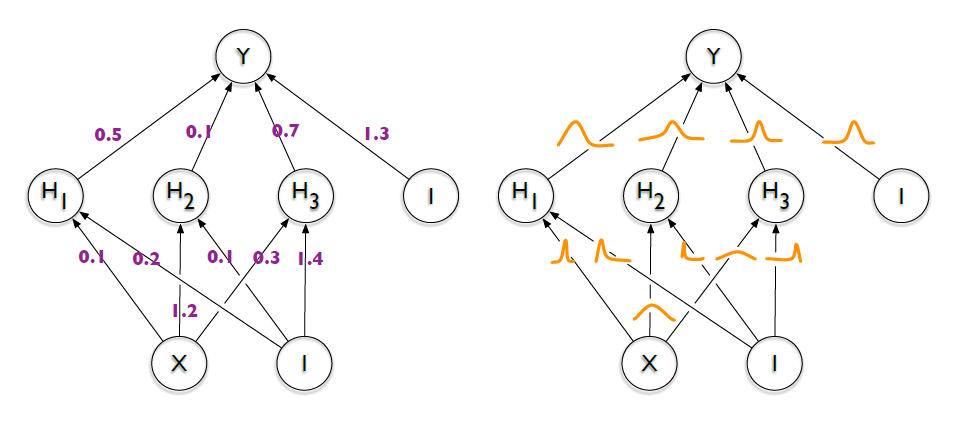
\includegraphics[width=0.6\textwidth]{image.png}
    \caption{On the left, each weight has a fixed value as provided by classical backpropagation. $^{[1]}$}
\end{figure}

\section{Bayesian Neural Networks and Variational Inference}

\textbf{Bayesian Neural Networks (BNNs)} provide a principled framework for modeling uncertainty in neural network parameters. They assign probability distributions to the weights and biases of a neural network, enabling us to capture uncertainty and make probabilistic inferences. In BNNs, model parameters, denoted as $\theta$, are treated as random variables, following a probability distribution $P(\theta)$. The goal is to infer the posterior distribution $P(\theta|D)$ over these parameters given observed data $D$.

However, exact Bayesian inference can become prohibitively expensive for complex models due to the need to enumerate over a vast parameter space.

\textbf{Variational Inference} offers an approximation approach to Bayesian inference. It approximates the complex posterior distribution $P(\theta|D)$ with a simpler, tractable distribution $Q(\theta)$. The primary idea is to optimize the parameters of $Q(\theta)$ to make it as close as possible to $P(\theta|D)$ while ensuring computational efficiency.

\textbf{The Core Elements of Variational Inference}:

\textbf{Evidence Lower Bound (ELBO):}
The ELBO, denoted as $L(\theta, q)$, is a crucial quantity in Variational Inference. It serves as a lower bound on the log-evidence $\log[P(D)]$, representing the likelihood of the data $D$:

\[L(\theta, q) = \log[P(D)]\]

The ELBO can be decomposed into two parts: a data fidelity term and a divergence term.

\textbf{Data Fidelity Term:}
The data fidelity term is typically the negative of the expected loss under the variational distribution $Q(\theta)$:

\[-\int q(\theta)\log[P(D|\theta)]d\theta\]

For regression tasks, this term often corresponds to a mean squared error (MSE) loss, while for classification tasks, it can be linked to the cross-entropy loss.

\textbf{Divergence Term (KL Divergence):}
The KL divergence between the variational distribution $Q(\theta)$ and the prior distribution $P(\theta)$ measures the difference between these distributions:

\[\text{KL}(q(\theta) || p(\theta))\]

This term accounts for the regularization aspect of Variational Inference. It discourages $Q(\theta)$ from deviating too far from the prior $P(\theta)$. In this context, the prior is often assumed to be a simple distribution, such as a Gaussian.

\textbf{Objective Function:}
The overall objective in Variational Inference is to maximize the ELBO. This is equivalent to minimizing the negative ELBO, which can be expressed as:

\[-\text{ELBO} = -\int q(\theta)\log[P(D|\theta)]d\theta + \text{KL}(q(\theta) || p(\theta))\]

This optimization problem transforms the inference task into an optimization task.

\textbf{Stochastic Optimization:}
Variational Inference frequently relies on stochastic optimization techniques, such as stochastic gradient descent (SGD), to estimate the ELBO and iteratively update the variational distribution parameters to approximate the posterior distribution.

\textbf{The Challenge of High-Dimensional Posterior Space}:

\textbf{Enumeration-Based Approaches:}
Traditionally, exact Bayesian inference would require enumerating over an immense parameter space, exploring possible values for each parameter. For a neural network with millions of parameters, this is infeasible.

\textbf{Variational Bayes and "Well-Behaved" Distributions:}
Variational Bayes introduces a powerful concept—approximating the posterior with a "well-behaved" distribution. Such a distribution, often Gaussian, is characterized by a small set of parameters, e.g., mean ($\mu$) and variance ($\sigma^2$).

\textbf{Optimizing the Approximating Distribution:}
The parameters of this approximating distribution are optimized iteratively using gradient descent. The aim is to bring this distribution as close as possible to the true posterior distribution in terms of Kullback-Leibler divergence.

\[\text{KL}(Q(\theta) || P(\theta|D))\]

\textbf{The Role of Evidence Lower Bound (ELBO):}
The ELBO provides a measure of the closeness between $Q(\theta)$ and the true posterior, even when we do not have direct access to the posterior. This optimized approximating distribution can then be used to make predictions with quantified uncertainty.

In essence, Variational Inference, through Variational Bayes, brings practicality to Bayesian inference in high-dimensional spaces, enabling Bayesian Neural Networks to express uncertainty and provide meaningful predictions even when faced with previously unseen inputs.




\section{Variational BNN (Classification - MNIST Data)}

\begin{figure}[h]
  \centering
  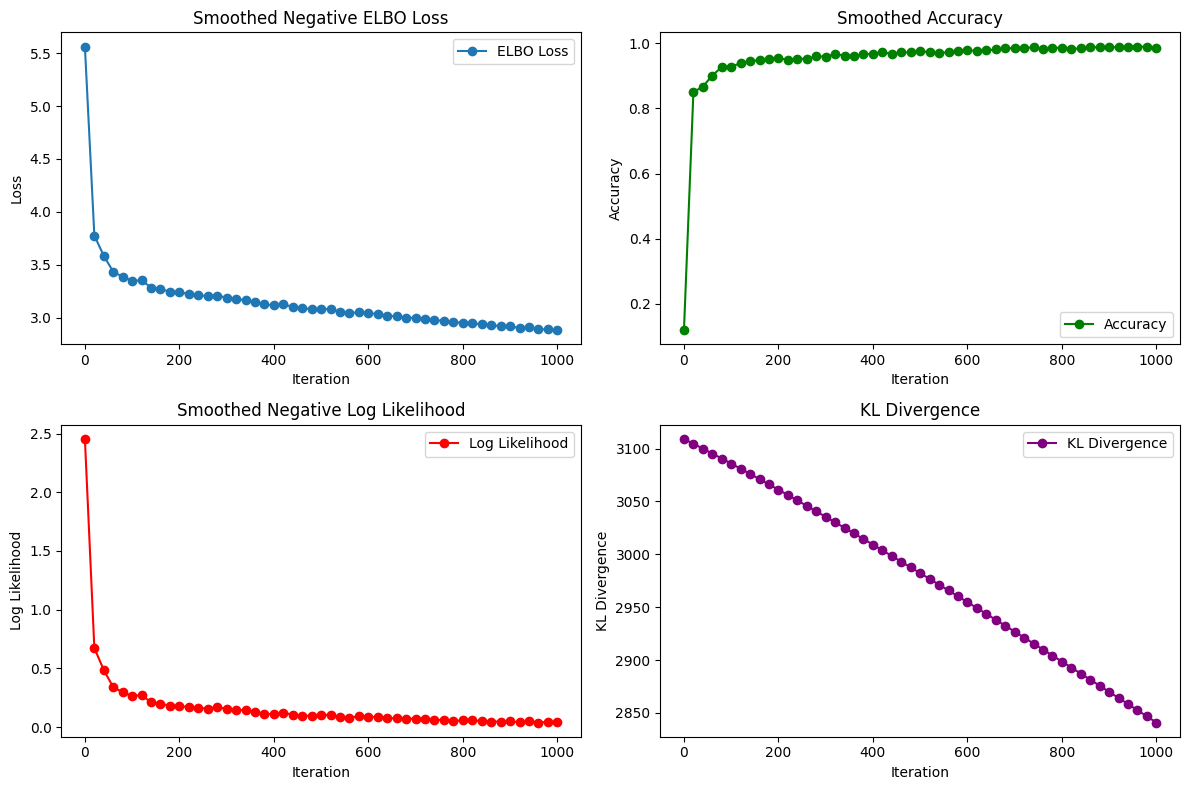
\includegraphics[width=0.8\textwidth]{download.png}  % Adjust the width as needed
  \caption{Plots of ELBO losses, Accuracy, Log Likelihood, and KL Divergence.}
  \label{fig:plots}
\end{figure}

\subsection{Dataset and Preprocessing}

The MNIST dataset consists of 28x28 grayscale images of handwritten digits (0-9). TensorFlow Datasets (TFDS) is used to download and preprocess the dataset.

\subsection{BNN Architecture and Configuration}
The BNN architecture is based on a multi-layer perceptron (MLP) model. It includes a single hidden layer with 1024 neurons and ReLU activation layer. The network is implemented using JAX and Haiku, making it compatible with Bayesian learning.

\subsection{Hyperparameter Tuning}
Hyperparameters play a crucial role in training BNNs. One vital hyperparameter is the factor applied to the KL divergence term within the Evidence Lower Bound (ELBO) loss. In this implementation, we set this factor to 0.001, aligning it with the initialization strategy. The careful tuning of this factor and the initialization scale is essential for a well-behaved BNN.

\subsection{Training the BNN}

Training a BNN involves several key steps:

\subsubsection{Initialize Bayesian NN Parameters}
The training begins by initializing the Bayesian NN parameters using the MLP model's parameters. These parameters are represented as a dictionary with 'mu' for means and 'logvar' for log-variance. This initialization is based on the mean-field approximation to the posterior, which represents the variational distribution as a Gaussian distribution with mean and variance (log-variance). This simplifies the training process, allowing sampling from a Gaussian distribution.

\subsubsection{Initialize the Optimizer}
The Adam optimizer is employed with a specified learning rate. It is initialized with the parameters from the previous step.

\subsubsection{Define the Evidence Lower Bound (ELBO) Objective}
The ELBO objective is defined to guide the training process. It consists of two main components:

\paragraph{Log Likelihood}
This term measures how well the model predicts the labels for a batch of images. It is computed using the softmax cross-entropy with logits.

\paragraph{Regularization Loss (KL Divergence)}
The KL divergence between the variational distribution (approximate posterior) and a normal distribution is calculated. This term acts as a regularization that encourages the approximate posterior to be close to the normal distribution.

The ELBO is computed as the combination of these two components, weighted by a hyperparameter (beta). The objective is to maximize the ELBO, which is equivalent to minimizing the negative ELBO. This process aligns with the concept of variational inference in Bayesian models.

\subsubsection{Training Loop}
The BNN is trained using stochastic gradient descent (SGD). The \texttt{sgd\_update} function is utilized to perform one step of SGD. It computes gradients using JAX's \texttt{grad} transformation and updates the model's parameters based on these gradients and the optimizer's state. The process repeats iteratively, gradually improving the model's performance.


\subsection{Prediction}
Predictions from the BNN are obtained by running predictions on multiple sets of parameters. This process helps in quantifying uncertainty. The predictions are averaged to get a final prediction, and the standard deviation of these predictions serves as a measure of uncertainty.

\subsection{Tuning for Training Success}
Achieving good training results with a BNN can be challenging. Two key tricks are discussed to make training more successful:

\subsubsection{Low Beta}
The hyperparameter 'beta' in the ELBO objective weighs the classification loss and regularization loss. Setting 'beta' too high can lead to strong regularization, hindering the model's ability to learn from the data. The recommended value is typically lower, such as 0.001, to prevent over-regularization.

\subsubsection{Low Initial Variance}
The initial variance of the variational distribution should be set carefully. A value that's too large can hinder the training process. In the discussed example, the variance was set to approximately 0.001, which is a suitable starting point for training.

\subsection{Training Results and Inferences}

After training the Bayesian Neural Network (BNN), we observed significant improvements in its performance at two different iterations:

\begin{table}[h]
\centering
\caption{BNN Evaluation Results}
\label{tab:bnn-eval}
\begin{tabular}{|l|l|l|l|l|l|}
\hline
\textbf{Iteration} & \textbf{Accuracy} & \textbf{ELBO} & \textbf{Log Likelihood} & \textbf{KL Divergence} & \textbf{Mean Approximate Evidence} \\
\hline
0 & 0.12000 & -5.56209 & -2.45310 & 3108.98438 & 0.57338 \\
\hline
1000 (Train) & 0.98700 & -2.88892 & -0.04794 & 2840.97729 & 0.74909 \\
\hline
1000 (Test) & 0.97900 & -2.91372 & -0.07274 & 2840.97729 & 0.74724 \\
\hline
\end{tabular}
\end{table}
\textbf{Inferences from Results:}

\begin{enumerate}
  \item \textbf{Accuracy Improvement:} The accuracy increased significantly , indicating a substantial enhancement in the model's ability to correctly classify MNIST digits, achieving nearly 0.99  accuracy.
  
  \item \textbf{ELBO Improvement:} The ELBO increased , indicating a better fit of the model to the data, demonstrating improved representation of the MNIST dataset after training.
  
  \item \textbf{Log Likelihood Improvement:} The log likelihood increased, suggesting that the BNN assigns higher probabilities to true labels, enhancing prediction quality.
  
  \item \textbf{KL Divergence Reduction:} The KL divergence decreased, indicating that the approximate posterior is closer to the normal distribution, reflecting less regularization and improved model stability.
  
  \item \textbf{Higher Mean Approximate Evidence:} The mean approximate evidence increased, signifying improved data fit and overall performance.
\end{enumerate}

In conclusion, these results highlight the effectiveness of BNN training. The model has evolved from an initial state of low accuracy and high regularization to a high-performing model with significantly improved accuracy and better data fit. Carefully tuned hyperparameters, such as the 'beta' parameter and initial variance, have played a crucial role in achieving this level of performance. The BNN is now capable of accurate digit classification and provides meaningful uncertainty estimates.




\section{Variational BNN (Regression on Sine Wave)}

\begin{figure}[h]
  \centering
  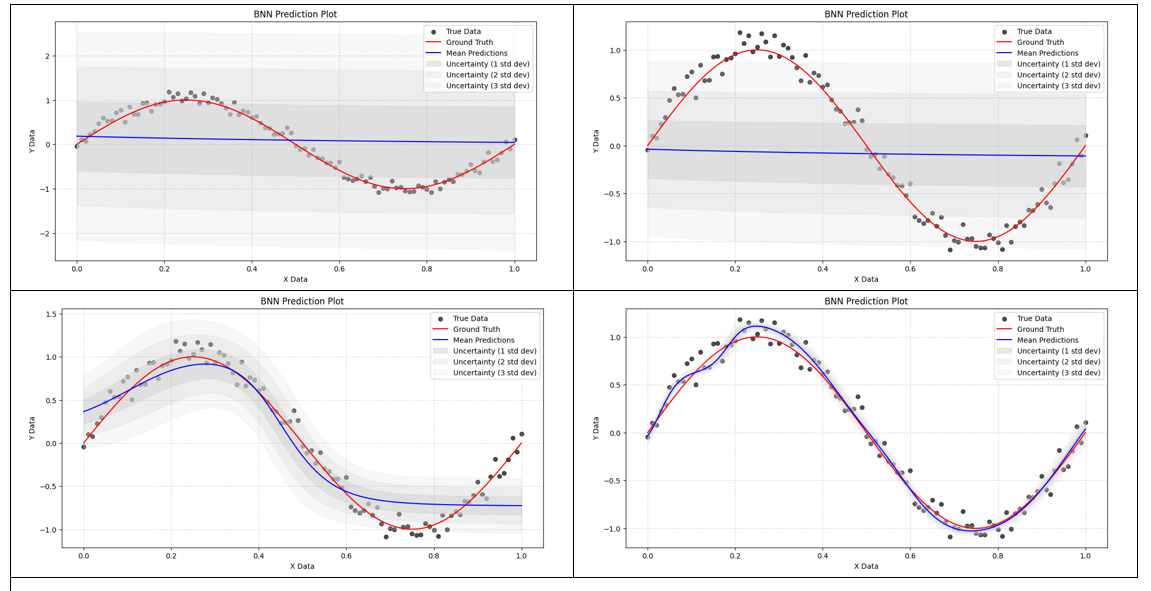
\includegraphics[width=0.8\textwidth]{pic1.png}
  \caption{Plots of Mean, Ground Truth, Data Points, and Uncertainty for beta = 1, 0.1, 0.01, 0.0001.}
  \label{fig:sine-wave-regression}
\end{figure}


\begin{figure}[h]
  \centering
  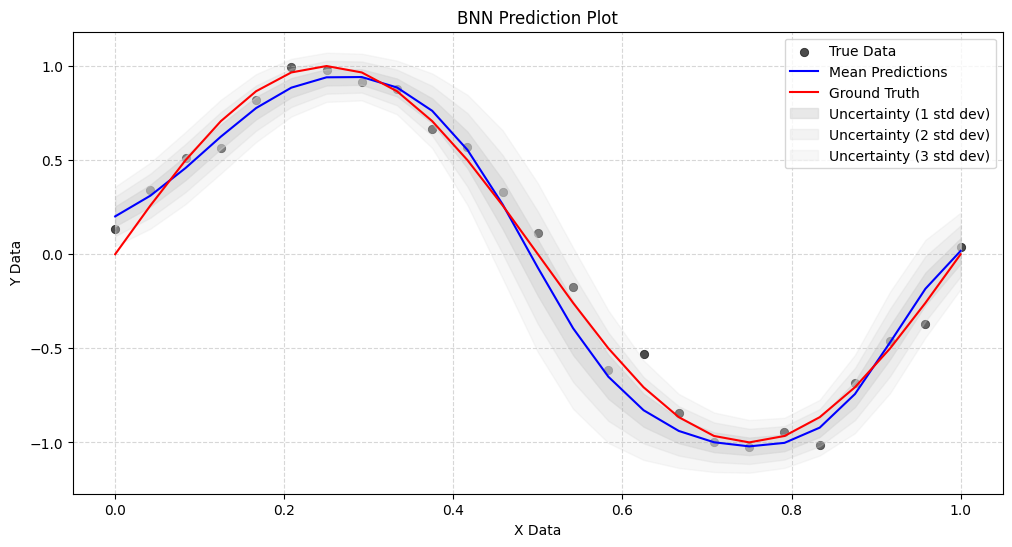
\includegraphics[width=0.8\textwidth]{reg.png}
  \caption{Plots of Mean, Ground Truth, Data Points, and Uncertainty for beta = 0.001.}
  \label{fig:sine-wave-regression}
\end{figure}

\subsection{Architecture and Hyperparameters}

The architecture and hyperparameters used for the sine wave regression task are 2 hidden layers with 10 neurons with tanh activation. The architecture details and hyperparameters are critical components in achieving the observed improvements in training results.


\subsection{Training Results and Analysis}

The BNN was trained on a sine wave regression task, and the following results were obtained at two different iterations:

\begin{table}[h]
\centering
\caption{BNN Evaluation Results at Different Iterations}
\label{tab:bnn-eval-iterations}
\begin{tabular}{|l|l|l|l|l|}
\hline
\textbf{Iteration} & \textbf{ELBO} & \textbf{L2 Loss} & \textbf{KL Divergence} & \textbf{Mean Approximate Evidence} \\
\hline
0 & -0.67635 & -0.60035 & 76.00484 & 0.93460 \\
\hline
50000 & -0.04507 & -0.01688 & 28.19097 & 0.99550 \\
\hline
\end{tabular}
\end{table}
\textbf{Analysis of Training Results:}

1. \textbf{ELBO Improvement:} The Evidence Lower Bound (ELBO) significantly improved from -0.67635 at iteration 0 to -0.04507 at iteration 50000. This indicates that the BNN is increasingly capturing the underlying patterns in the data, resulting in a better fit to the sine wave.

2. \textbf{L2 Loss Reduction:} The L2 loss improved from -0.60035 to -0.01688, indicating a reduction in the mean squared error between the BNN's predictions and the ground truth sine wave. This suggests a more accurate regression model.

3. \textbf{KL Divergence Reduction:} The KL Divergence decreased from 76.00484 to 28.19097. This reduction suggests that the approximate posterior distribution is approaching a normal distribution, indicating a decrease in model regularization.

4. \textbf{Higher Mean Approximate Evidence:} The mean approximate evidence increased from 0.93460 to 0.99550, implying an improved data fit and overall model performance. A higher value indicates a better match between the data and the model's parameters.

In conclusion, the BNN's performance on the sine wave regression task significantly improved during training. The results demonstrate that it learned to capture the underlying patterns in the data, resulting in a more accurate regression model with reduced uncertainty and increased data fit.


\section*{References}

{
\small

[1] Charles Blundell, Julien Cornebise, Koray Kavukcuoglu, and Daan Wierstra. Weight uncertainty in neural networks. arXiv preprint arXiv:1505.05424, 2015.

[2] Piero Esposito. Blitz - bayesian layers in torch zoo (a bayesian deep learning library for torch). 

\url{https://github.com/piEsposito/blitz-bayesian-deep-learning/}, 2020.

[3] 
Paras Chopra. Making Your Neural Network Say "I Don't Know": Bayesian NNs Using Pyro and PyTorch.


%%%%%%%%%%%%%%%%%%%%%%%%%%%%%%%%%%%%%%%%%%%%%%%%%%%%%%%%%%%%


\end{document}